\chapter{Рассеяния носителей на шероховатой поверхности} \label{chapt1}

\section{Обзор литературы} \label{sect1_1}
Фактически первыми на важную роль взаимодействия носителей с шероховатой поверхностью в процессах переноса обратили внимание H. Sakaki и др. \cite{Sakaki1987} при исследовании подвижности в КЯ GaAs/AlAs малой толщины ($40\AA$, $60\AA$). При этом подвижность оказалась очень чувствительной величиной от ширины $a$ квантовой ямы. При низких температурах $(T = 4.2 K)$ подвижность при  $a < 60 \AA$ с ростом толщины увеличивалась как $a^{6}$. Для описания экспериментальных данных по величине и температурной зависимости подвижности в кремниевых инверсионных слоях $(\text{Si-SiO}_2)$ в области низких температур $(T\le 80 \text{K})$ параметры флуктуирующей поверхности принимают значения $\Delta = 6\AA$, $\Lambda = 13\AA$ \cite{Stern1980, Cham1980}. Как показали теоретические и экспериментальные исследования в КЯ GaAs/AlAs \cite{Unuma2001}, влияние рассеяния носителей на шероховатой поверхности на подвижность и полуширину линии при межподзонных оптических переходах существенно вплоть до комнатных температур (толщина $a \cong 80 \AA$). В \cite{Leuliet2006} при исследовании оптических свойств сверхрешеток с активной областью GaAs/AlGaAs показано, что в отсутствии магнитного поля рассеяние носителей на шероховатой поверхности всегда доминирует в области низких температур над другими механизмами рассеяния (рассеяние на длинноволновых акустических фононах, на примесях). В работе \cite{Gold1990} рассматривалось влияние рассеяния носителей на шероховатой поверхности на подвижность вырожденного электронного газа в квантовых проволоках цилиндрической формы с бесконечным потенциалом на границе $r=R_0 $. На влияние рассеяния носителей на шероховатой поверхности на форму фотолюминесценции было обращено внимание в \cite{Gurioli1991}. Влияние электрического поля $E$, направленного перпендикулярно поверхности прямоугольной квантовой ямы, на рассеяние носителей на шероховатой поверхности (в случае гауссовской флуктуации поверхности) исследовалось в \cite{Ibragimov2002}. Было показано, что вероятность рассеяния в единицу времени увеличивается с ростом $E$ (при $E>3\cdot 10^5 \text{V/cm}$ это увеличение для КЯ с шириной $60 \AA$ более чем в три раза).

Теоретические расчеты времени релаксации (транспортного времени) с учетом рассеяния носителей на шероховатой поверхности (surface roughness scattering) для описания температурной зависимости подвижности в инверсионных слоях кремния проводились в \cite{Stern1980,Masaki1989}.

В работе \cite{Motohisa1992} обсуждалось влияние рассеяния носителей на шероховатой поверхности на подвижность в квантовых проволоках, когда электроны находятся в нижайшей подзоне. В \cite{Tsetseri2004,Tsetseri2008} исследовалось поведение подвижности в области низких температур в Al-GaAs/GaAs $V$-подобной квантовой проволоке, когда учитывалось рассеяние на шероховатой поверхности. Рассеяние расчитывалось для концентрации электронов равной $10^6 \mathrm{cm^{−1}}$ и температуре $40К$ с использованием золотого правила Ферми. Было определенно, что рассеяние на акустических фононах пренебрежимо мало при температурах $T<4K$ и становится заметным при $T>10K$, а рассеяние на шероховатой поверхности и на равномерно распределенных примесях являются доминирующими механизмами рассеяния.
В \cite{Vurgaftman1997} авторы обратили внимание на влияние этого механизма на внутри- и межподзонные переходы ($\Delta =10\AA$, $\Lambda =30 \AA$) для вырожденного электронного газа. В исследованиях \cite{Quang2006} проводились расчеты транспортного времени релаксации в гетероструктурах для прямоугольной квантовой ямы конечной высоты барьера на границе $\mathrm{ A_{x}Ge_{1-x}N/GeN}$ с малой плотностью носителей с учетом рассеяния и на шероховатой поверхности.
Исследование ограничения низкотемператруной $(1.5 \mathrm{K})$ подвижности в гетероструктурах AlGaAs/GaAs проводилось в \cite{Saku1996,Saku1991}, получены подвижности порядка $10^7 \frac{\text{cm}^{-2}}{\text{Vs}}$, авторы указывают на то, что рассеяние носителей на ионизированных примесях и шерохватой поверхности доминируют в ограничении подвижности при низких температурах.

В работе \cite{Borzdov2007} теоретически исследовалось, в частности, влияние рассеяния электронов на шероховатой поверхности в транзисторной структуре на основе квантовой проволоки GaAs в матрице AlAs. Влияние рассеяния электронов на шероховатой поверхности на явления переноса в полупроводниковых графитовых нанолентах изучалось в \cite{Fang2008}. В этой работе, в частности, обсуждается вопрос локализации носителей на шероховатой поверхности при больших значениях $\Delta, \Lambda$ флуктуирующей поверхности. В \cite{Kamalakar2009} обсуждалась роль рассеяния носителей на поверхности на низкотемпературные явления переноса в Ni нанопроволоках (диаметр проволоки изменяется от 13 до 55 nm). С ростом диаметра квантовой проволоки при низких температурах влияние поверхности на удельное сопротивление, как показывают экспериментальные исследования, уменьшается и отклонение удельного сопротивления от объемного материала уменьшается. Влияние шероховатой поверхности с различной шириной шероховатости ($\Lambda $ менялось от $13 \AA$  до $108 \AA$) на теплопроводность в нанопроволоках кремния экспериментально исследовалось в \cite{Liu2010}. Было показано, что с увеличением неровностей поверхности исследуемой наноструктуры теплопроводность уменьшается.

Температурная зависимость электропроводности нанопроволок из монокристаллического германия экспериментально рассматривалась в работе \cite{Gu2001}. Показано что с уменьшением температуры сопротивление заметно возрастает. Такая температурная зависимость сопротивления говорит об уменьшении подвижности связанное с рассеянием носителей на шероховатой поверхности.

Различные механизмы рассения носителей в поликристаллических и монокристаллических тонких пленках и нанопроволоках меди экспериментально исследовалось в \cite{Chawla2011}. Приведены зависимости различных величин от размеров наноструктур. Указывается на отклонение от правила Маттисена при учете различных механизмов рассеяния.

В \cite{Lal2003} теоретически исследовалось (формула Кубо) влияние электрон-фононного взаимодействия на электропроводность в металлических нанопроволоках. Была изучена зависимость сопротивления от толщины проволоки, температуры и энергии Ферми. Показано, что удельное сопротивление увеличивается с уменьшением толщины проволоки. Температурная зависимость показывает линейную зависимость для проволок толщиной <~20~nm.

В \cite{Arutyunayan2010} рассматривалось влияние сильного внешнего однородного электрического поля на внутризонные переходы в квантованном цилиндрическом слое в приближении изотропной эффективной массы. Показано, что сильное внешнее электрическое поле приводит к дополнительной локализации носителей по их угловому движению.
Подвижность ультра тонких квантовых каналов (меньше 20 nm) зажатых между различными оксидным затворами с использованием численного моделирования исследовалась в \cite{Krivec2016}. Сравнивалась подвижность различно ориентированных структур. Ориентация поверхности (111) в InGaAs дает улучшение подвижности по сравнению с (100)-ориентированным устройством, независимо от толщины структуры.

В \cite{Thongnum2008} вычислена плотность состояний 2D электронного газа в размерно-ограниченных квантовых ямах с учетом шероховатой поверхности.  Показано что плотность 2D состояний зависит от флуктуации потенциала (среднеквадратичной). Шероховатость поверхности вызывает локализованные состояния ниже края подзоны проводимости.

Влияние шероховатой поверхности на оптическое пропускание света через многослойные полимерные пленки рассмотрено в \cite{Larena2002}. Показана сильная зависимость между спектральными параметрами оптического пропускания и шероховатой поверхности.

С учетом фононного удержания в цилиндрической квантовой проволоке в диэлектрической среде на рассеяние электронов проведены расчеты в работе \cite{Vartanian2003}. Получены аналитические выражения для скоростей межподзонного рассеяния. Показано что учет фононного удержания приводит к увеличению подвижности.

В \cite{Lizzit2013} предложен подход для моделирования подвижности ограниченной рассеянием носителей на шероховатой поверхности в МОП транзисторах.

В \cite{Myronov2008a,Myronov2008,Mironov2014,Myronov2015} получены Ge квантовые ямы, с проводимостью двумерного дырочного газа в три раза выше стандартной при комнатных температурах. Улучшение было получено за счет модификации профиля валентной зоны, исследована зависимость проводимости от магнитного поля при комнатных температурах. Указывается на то что температурная зависимость подвижности различна в области низких температур в структурах DS-MOD и SS-MOD, что связано с разным качеством поверхности этих структур.

В \cite{Shin2015} определялись характеристики FD-SOI устройств n-типа выполненных по 14 nm технологии методом магнетосопротивления. Показано что для длинных каналов кулоновское рассеяние не играет существенной роли при комнатной температуре (приведены графики зависимости подвижности от плотности носителей). Указывается на влияние поперечного электрического поля на взаимодействие носителей с шероховатой поверхностью. 

В \cite{Moraga2015} вычислена электропроводность металлического образца под действием распределенных примесей и случайно-распределённой границы с помощью квантово-механической процедуры, основанной на формуле Кубо. Граница в виде одномерного массива дельтообразных потенциалов (Mayadas and Shatzke модель). Получено что, подвижность носителей в размерно-ограниченных системах ниже чем в объемных. В случае достаточно тонких образцов и достаточно большой шероховатости все носители заряда локализуются и проводимость падает до нуля. Так же указывается, что в квазиклассической модели, поток электронов рассеивается на каждом зерне шероховатости поверхности, тогда как в квантовомеханической модели нет частичного рассеяния. Аналогичные исследования проводились в \cite{Arenas2015}.

В \cite{Sonnet2011} экспериментально исследована подвижность электронов в In0.53Ga0.47As MOSFET инверсионных слоях. Пик подвижности электронов сильно зависит от подготовки поверхности. Подробный анализ подвижности в зависимости от электрического поля, легирования подложки и температуры позволил определить различные компоненты подвижности (подвижность ограниченную рассеянием на шероховатой поверхности, на фононах, кулоновских рассеянием).

В \cite{Kucek2015} экспериментально исследовались температурные зависисмости термоЭДС, электропроводности и др. кинетических коэффициентов в образцах Cu1−xNixInTe2

В \cite{Galagali2015} исследовались термоэлектрические свойства: подвижность, диффузионная термоЭДС и электронная термопроводимость в ZnO и GaN нанопроволоках при температурах 10<T<300 K. Представлены численные расчеты подвижности ограниченной рассеянием на акустических фононах, в приближении упругого рассеяния.

В \cite{Khanh2013} исследована зависимость транспортных свойств от концентрации носителей, толщины слоя, магнитного поля и температуры с учетом рассеяния на шероховатой поверхности. Результаты могут быть использованы для получения информации о механизмах рассеяния в квантовых яме SiGe/Si/SiGe, а в \cite{Tai2015} GaP/AlP/GaP квантовой яме.

В \cite{Condrea2010} измерялось сопротивления нанопроволок висмута различного диаметра и качества при одноосной деформации. Найдены колебания зависимости сопротивления при T=4.2K которые уменьшаются при T=77K.

Влияние шероховатой поверхности в квантовых ямах GaAs/AlAs на дефазировку блоховских осцилляций исследовалось в работах \cite{Unuma2006,Unuma2007}. Время дефазировки в таких структурах в режиме Ваннье-Штарка быстро уменьшается с уменьшением ширины квантовой ямы, такая сильная зависимость времени дефазировки от толщины ямы указывает на то что доминирующим механизмом дефазировки является шеровховатая поверхность раздела.

В \cite{Prunnila2005} исследовалась подвижность электронов в ультратонких двухстворчатых кремниевых MOSFET каналах, была обнаружена небольшая ассимитричность в подвижности между верхним и нижним каналом структуры, которая объясняется разностью в качестве поверхности каналов.

В \cite{Shchurova2009} рассчитывали температурную зависимость сопротивления Mn-DOPED GaAs / InGaAs / GaAs квантовых ям с учетом рассеяния носителей на шероховатой поверхности, исследована температурная зависимость, показано что при низких температурах сопротивление определяется spin-flip рассеянием и рассеянием на шероховатой поверхности, при увеличении температуры сопротивление растет и в основном определяется рассеянием на фононах, а также найдено отрицательное магнетосопротивление.

В \cite{Lee2011b} экспериментально исследовано влияние поверхности на подвижность носителей при низких температурах, указано что совершенствование процесса травления позволит улучшать проводимость при низких температурах.

В \cite{Penner1999} указывается что рассеяние на шероховатой поверхности может преобладать над всем остальными типами рассеяния при низких температурах для квантовых ям размером меньше 100 ангстрем.

Исследованием влияние поверхности на подвижность в полупроводниковых гетероструктурах занимались в \cite{Feenstra1995}, найдено значительно уменьшение подвижности при увеличении шероховатости поверхности.

В \cite{Yutani1996} измерили подвижность электронов в Si КЯ как функцию ширины квантовой ямы и получили монотонное уменьшение подвижности с уменьшением ширины ямы.

Исследование распределения шероховатой поверхности в буферном слое SiGe с вложенными в него слоями Si проводилось в \cite{Yoon2005} показана возможность сглаживания поверхности путем вставки напряженно-деформированных слоев Si в процессе роста слоя SiGe.

В \cite{Tito2017} учитывали рассеяние на шероховатой поверхности при определения края подвижности, указывается на то, что в тонких квантовых ямах шероховатая поверхность сильно влияет на локализацию носителей


\section{Теория рассеяния носителей на шероховатой поверхности в размерно-ограниченных системах} \label{sect1_2}
Модель взаимодействия носителей с шероховатой поверхностью строится следующим образом: из-за неровности поверхности случайным образом меняется ширина $a$ размерно-ограниченной системы, что приводит к флуктуации энергии размерного квантования $E_{\alpha}$ при движении носителя параллельно поверхности исследуемой квантовой системы. Следовательно, энергия взаимодействия электрона (дырки) с шероховатой поверхностью в случае двухмерного электронного газа может быть записана в следующем виде \cite{Sakaki1987}:
\begin{equation}
\label{eq:1_1}
V(x,y)=\frac{\partial E_{\alpha}}{\partial a}\Delta(x,y)\equiv V_{\alpha} \Delta(x,y)
\end{equation}
$\Delta(x,y)$ --- случайная функция.

Например, для прямоугольной квантовой ямы (КЯ) с бесконечными стенками для потенциала:
\begin{equation}
\label{eq:1_2}
E_n = \frac{\hbar^2 \pi^2 n^2}{2ma^2} \equiv E_0 n^2 \Rightarrow V_n = -\frac{2}{a}E_0 n^2
\end{equation}

Для случая квантовой ямы с параболическим потенциалом для электрона с эффективной массой $m_e$:
\begin{equation}
\label{eq:1_3}
E_n=2\hbar \left[ \frac{2\Delta E_c} {m_e} \right]^\frac{1}{2} \frac{1}{a}\left( n + \frac{1}{2} \right) = \hbar \omega_e \left( n + \frac{1}{2} \right), V_n = -\frac{1}{a} \hbar \omega_e \left( n + \frac{1}{2} \right)
\end{equation}
$\Delta E_c$ --- высота параболического потенциала на границе наноструктуры, $\hbar \omega_e$ --- энергия размерного квантования.

Часто при расчетах кинетических коэффициентов используется случай гауссовой флуктуации поверхности, когда автокорреляционная функция для различных точек поверхности определяется соотношением \cite{Sakaki1987,Shchurova2009,Pozdnyakov2006,Khanh2016,Gold1987,Thongnum2008,Su2013}:
\begin{equation}
\label{eq:1_4}
\left\{ \Delta(x,y)\Delta(x',y') \right\}_V = \Delta^2 \exp \left[ - \frac{1}{\Lambda^2} \left( (x-x')^2 +(y-y')^2 \right) \right] \equiv F \left( \left| \boldsymbol{\rho} - \boldsymbol{\rho'} \right| \right),
\end{equation}
здесь:
$\Delta, \Lambda$ --- высота и ширина гауссовой флуктуации соответственно, 
$\left\{ ... \right\}_V$
описывает усреднение по реализации случайного процесса 
$\Delta(x,y)$, $\left| \vect{\rho} - \vect{\rho'} \right| = \sqrt{(x-x')^2 + (y-y')^2}$.
Естественно, что можно рассматривать случай $\delta$-образной флуктуации \cite{Lozovik1998}, когда
\begin{equation}
\label{eq:1_5}
\left\{ \Delta(x,y)\Delta(x',y') \right\} = \gamma\delta\left( \boldsymbol{\rho} - \boldsymbol{\rho'} \right) = \gamma_0\delta(x-x')(y-y')=\tilde{F} \left(\left| \boldsymbol{\rho} - \boldsymbol{\rho'} \right|\right)
\end{equation}
$\gamma_0$ определяет квадрат амплитуды флуктуации.

Если исследовать случай одномерного электронного газа (примером могут служить квантовые проволоки, квантовые нанотрубки), то для гауссовой флуктуации поверхности автокорреляционная функция для различных точек поверхности по аналогии (\ref{eq:1_4}) может быть записана следующим образом:
\begin{equation}
\label{eq:1_6}
\left\{\Delta(x)\Delta(x')\right\}=\Delta^2_0 \exp \left[-\frac{(x-x')^2}{\Lambda^2_0}\right] = F_0(x-x')
\end{equation}
Для случая $\delta$-образной флуктуации поверхности естественно положить:
\begin{equation}
\label{eq:1_7}
\left\{\Delta(x)\Delta(x')\right\}= \gamma\delta(x-x') = \tilde{F}_0(x-x')
\end{equation}

Время релаксации носителей на шероховатой поверхности определяемое квантово-механической вероятностью рассеяния в единицу времени, в нижайшем порядке теории возмущений определяется соотношениями \eqref{eq:31_140}, \eqref{eq:31_85}:
\begin{equation} \label{eq:1_8}
\frac{1}{\tau_a}=\frac{2\pi}{\hbar} \sum_\beta{W_{\alpha\beta}\delta\left(\varepsilon_\alpha-\varepsilon_\beta\right)}
\end{equation}
\begin{equation} \label{eq:1_8_5}
W_{\alpha\beta}=\int{d\vect{r} d\vect{r_1} \Psi^*_\alpha(\vect{r}) \Psi^*_\beta(\vect{r_1}) V_\alpha V_\beta F \Psi_\alpha(\vect{r_1}) \Psi_\beta(\vect{r})}
\end{equation}
$\Psi_\alpha(\vect{r_1})$--- волновая функция носителей в состоянии $\alpha$ в размерно-квантованной системе. $F$ определяется соотношением (\labelcref{eq:1_4,eq:1_5,eq:1_6,eq:1_7}).

Для квазидвумерных систем с бесконечным потенциалом (квантовые ямы, гетероструктуры) в случае гауссовой флуктуации поверхности (\ref{eq:1_4}) нетрудно получить:
\begin{equation} \label{eq:1_9_0}
W_{\alpha\beta} =\frac{\pi }{L_x L_y} (\Delta \Lambda )^2 V_{\alpha} V_{\beta } \exp \left[-\frac{\Lambda^2 }{4} \left|k_{\bot } -k'_{\bot } \right|^2 \right],
\end{equation}
и время релаксации при рассеянии носителей в одной зоне определяется соотношением:
\begin{equation} \label{eq:1_9}
\frac{1}{\tau_a}=\frac{m_e}{\hbar^3}\pi{(\Delta \Lambda)}^2 V_n^2 \exp{\left[-\frac{1}{2}(\Lambda k_\bot )^2\right]} \mathrm{I}_0 \left[\frac{1}{2}(\Lambda k_\bot)^2\right]
\end{equation}
$\mathrm{I}_0(z)$~---~модифицированная функция Бесселя нулевого значка \cite{Abramowitz1979}, $k_\bot = \sqrt{k^2_x+k^2_y}$~---~волновой вектор электрона в плоскости двумерной системы.

При низких температурах, когда $\Lambda k_\bot \ll 1$ из (\ref{eq:1_9}) следует:
\begin{equation} \label{eq:1_10}
\frac{1}{\tau_a}=\frac{m_e }{\hbar^3}\pi (\Delta \Lambda)^2 V_n^2
\end{equation}
Аналогично можно записать для случая $\delta$-образной флуктуации поверхности
\begin{equation} \label{eq:1_11}
\frac{1}{\tau_a}=\frac{m_e}{\hbar^3}\gamma_0 V_n^2
\end{equation}
Согласно (\ref{eq:1_10}), (\ref{eq:1_11}) рассеяние электронов происходит в одной зоне, и время релаксации зависит только от номера размерно-квантованной зоны $n$. При этом с ростом $n$ $\tau_a$, если учитывать (\ref{eq:1_2}), (\ref{eq:1_3}), уменьшается.

В случае прямоугольной квантовой ямы:
\begin{equation}
\frac{1}{\tau_\alpha} \sim \frac{E_0^2}{a^2} n^4 
\end{equation}
А для параболической квантовой ямы:
\begin{equation} \label{eq:1_14}
\frac{1}{\tau_\alpha} \sim \frac{(\hbar\omega_e)^2}{a^2}{\left(n + \frac{1}{2}\right)}^2
\end{equation}
Следовательно, для двумерного электронного газа при низких температурах, время релаксации при рассеянии носителей на шероховатой поверхности \eqref{eq:1_10}, \eqref{eq:1_11} справедливо для произвольного вида потенциала $V(\vect{\rho})$:
\[
\left[-\frac{\hbar^2}{2m_e}\frac{\partial^2}{\partial \vect{\rho}^2}+V(\vect{\rho})\right]\Psi_n(\vect{\rho})=E_n\Psi_n(\vect{\rho}).
\]

Для одномерных квантовых систем (например, нанопроволоки, нанотрубки), когда носители свободно движутся вдоль оси $OX$ исследуемой наноструктуры, волновая функция определяется как
\[
\psi_\alpha(\vect{r})=Ce^{ik_x}\varphi(y,z),
\]
согласно \eqref{eq:1_8} для гауссовой флуктуации поверхности
\begin{equation}
W_{\alpha\beta }=\frac{\sqrt{\pi}\Delta^2_0\Lambda_0}{L_x}  V_n^2 \exp\left[-\frac{(k_x-k'_x)^2\Lambda^2_0}{4}\right] \delta_{nn'},
\end{equation}
для $\delta$-образной флуктуации поверхности
\begin{equation}
W_{\alpha\beta }=\frac{\gamma_0}{L_x} V_n^2 \delta_{nn'}.
\end{equation}
Наличие символов Кронекера указывает, что процессы рассеяния носителей происходят в одной зоне. Следовательно, согласно \eqref{eq:1_8} время релаксации определяется соотношением
\begin{equation} \label{eq:1_15_5}
\frac{1}{\tau_\alpha}=\frac{L_x}{\hbar }\sum\limits_{n_1}\int\limits^\infty_{-\infty }{W_{n k_x, n_1 k'_x}\delta(\varepsilon_{n k_x}-\varepsilon_{n_1 k'_x})dk'_x}.
\end{equation}
Тогда для квадратичного закона дисперсии
\[
\varepsilon(k_x)=\frac{\hbar^2 k^2_x}{2m_e} 
\] 
и гауссовой флуктуации поверхности \eqref{eq:1_6}, из \eqref{eq:1_15_5} нетрудно получить  
\begin{equation} \label{eq:1_16}
\frac{1}{\tau_\alpha}=\frac{2 m_e}{\hbar^3} \frac{V_n^2}{\left|k_x\right|} \frac{\Delta^2_0\Lambda_0\sqrt{\pi}}{2} \left(1+\exp\left[-\Lambda^2_0 k^2_x \right] \right)
\end{equation}
аналогично для $\delta$-образной флуктуации поверхности \eqref{eq:1_7}, время релаксации имеет вид:
\begin{equation} \label{eq:1_17}
\frac{1}{\tau_\alpha}=\frac{2 m_e}{\hbar^3} \frac{V_n^2}{\left|k_x\right|}\gamma_0
\end{equation}

Из \eqref{eq:1_16} и \eqref{eq:1_17} следует что, время релаксации зависит от номера размерно-квантованной зоны и имеет особенности при $k_x=0$, т.е. на дне зоны проводимости. Последнее обстоятельство является непосредственным следствием одномерности движения носителей заряда. 

Особый интерес представляют наноструктуры в поперечном электрическом поле, которое существенно влияет на явления переноса в наноструктурах. В параболических квантовых ямах (ПКЯ), когда постоянное электрическое поле $E$ направлено вдоль оси пространственного квантования, потенциальная энергия электрона определяется соотношением:
\[
U(z)=\frac{m_e \omega^2 }{2} z^2 +eEz.
\]
Волновая функция и собственные значения энергии электрона уравнения Шредингера с потенциальной энергией $U(z)$ известна \cite{Sinyavskii1998}:
\begin{equation}
\Psi^{(c)}_{k_x,n,m}(x,y,z)=\frac{e^{ik_x x}}{\sqrt{L_x}}\frac{e^{ik_y y}}{\sqrt{L_y}}{\left(\frac{\lambda }{\pi}\right)}^{\frac{1}{4}}\frac{1}{\sqrt{2^nn!}}H_n\left[(z-z_0)\sqrt{\lambda }\right]e^{-\frac{\lambda }{2}(z-z_0)^2},
\end{equation}
\[
\lambda =\frac{m_e\omega }{\hbar},\;
z^{(c)}_0 = -\frac{eF}{m{\omega }^2}.
\]
\begin{equation} \label{eq:41_10}
E_{n,k_{\bot } } =\frac{\hbar^2 k_{\bot }^2 }{2m_c} +E_n,
\end{equation}
\[
E_n =\hbar \omega \left(n+\frac{1}{2} \right)-\Delta_c, \;
k_{\bot }^2 =k_x^2 +k_y^2,
\]
\begin{equation} \label{eq:41_15}
\Delta_c =\frac{e^2 E^2 }{2m_e \omega^2},
\end{equation}
$\hbar \omega $ -- энергия размерного квантования, которая простым образом связана с величиной потенциальной энергии $\Delta E_c$ на границе ПКЯ с шириной $a$
\[
\hbar \omega =\frac{2\hbar }{a} \sqrt{\frac{2\Delta E_c }{m_e} }.
\]
Заметим, что энергия размерного квантования убывает как $a^-1$  (в прямоугольных квантовых ямах она уменьшается как  $a^-2$).  
$k_{\bot } $~---~волновой вектор электрона в плоскости низкоразмерной системы, $\Delta_c$~---~энергия взаимодействия электрона с поперечным электрическим полем.
Для типичных параметров ПКЯ $\Delta E_c \sim 0.25\text{ eV} $ при $a=10^3 \AA$ $\hbar\omega = 14.5 \text{ meV}$ , т.е при $T \ll 170 \text{ K}$  исследуемая система является квантовой). Исследования кинетических и оптических явлений в размерно-ограниченных системах с использованием параболического потенциала широко проводятся в настоящее время \cite{Moldoveanu2010,Gusev2010}.

\begin{figure}[!h] 
	\center
	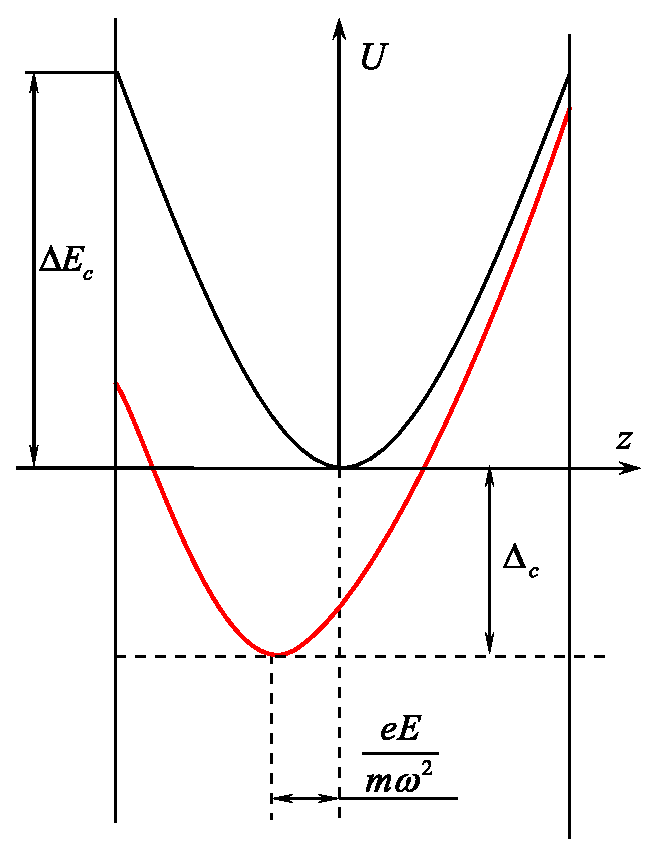
\includegraphics [scale=0.75] {fig_1_2_1}
	\caption{Потенциальная энергия параболической квантовой ямы в поперечном электрическом поле} 
	\label{img:fig_1_2_1} 
\end{figure}

Из энергетического спектра \eqref{eq:41_10} следует что с ростом напряженности электрического поля, минимум зоны проводимости опускается в область запрещенной зоны на величину $\Delta _{c} $ рисунок~\ref{img:fig_1_2_1} . В дальнейшем рассматриваем такие значения напряженности поперечного электрического поля $E$, при которых параболическая форма потенциальной энергии сохраняется, и в ней остается много размерно-квантованных эквидистантных уровней, т.е. решения уравнения Шредингера с потенциальной энергией $U(z)$ остаются справедливыми \cite{Kanarovskii1995}. Для параметров ПКЯ приведенных выше $E\le 3\cdot 10^4\text{ V/cm}$. При низких температурах $T$ в нелегированных системах с пониженной размерностью важным является механизм рассеяния носителей на шероховатой поверхности \cite{Sakaki1987,Vurgaftman1999}. В направлениях OX, OY свободного движения носителей заряда ширина ПКЯ изменяется случайным образом, и, следовательно энергия размерного квантования $E_n$, определяемая шириной квантовой системы, флуктуирует. Именно по этой причине энергию взаимодействия носителей с шероховатой поверхностью можно записать следующим образом \eqref{eq:1_1}:
\begin{equation} \label{eq:41_20}
W_{n} =\frac{\partial E_n }{\partial a} \Delta(x,y) \equiv -\frac{1}{a} \left[ E_n +2\Delta_c \right] \Delta (x,y)=V_n \Delta (x,y).
\end{equation}
Здесь $\Delta (x,y)$~---~случайная величина, автокорреляционная функция которой определяется: в случае гауссовой флуктуации поверхности выражением \eqref{eq:1_4}, в случае $\delta$-образной флуктуации поверхности выражением \eqref{eq:1_5}.

Необходимо заметить что в энергии \eqref{eq:41_10}, слагаемое отвечающее за взаимодействие носителя с поперечным электрическим полем зависит от энергии размерного квантования \eqref{eq:41_15}, которая непосредственно связана с шириной размерно-ограниченной системы, что приводит к дополнительному слагаемому $2\Delta_c / a$ в энергии взаимодействия носителя с шероховатой поверхностью \eqref{eq:41_20}. Такая зависимость механизма рассеяния от величины электрического поля представляется довольно интересной, т.к. другие мех анизмы рассеяния (на акустических фононах, на примесях) не зависят от величины поперечного электрического поля.

В случае $\delta $-образной флуктуации поверхности получаем
\begin{equation} \label{eq:41_70}
\frac{1}{\tau _{\alpha } } =\frac{\gamma_0 m_e (\hbar\omega_e)^2 }{\hbar^3 a^2 } \left[\left(n+\frac{1}{2} \right)+N_c \right]^2, \;
N_c =\frac{2\Delta_c }{\hbar \omega } .
\end{equation}  
заметим что в отсутствии электрического поля $(N_c = 0)$ из \eqref{eq:41_70} получаются результаты \eqref{eq:1_14}.

При расчете времени релаксации в случае гауссовской флуктуации поверхности, когда
\[
\frac{\hbar^2 }{2m} \Lambda^{-2} \gg (3/2)k_0 T ,
\]
что выполняется в широкой области температур, $1 / \tau_{\alpha }$ описывается соотношением \eqref{eq:41_70}, в котором нужно $\gamma_0 $ заменить на $(\pi \Delta^2 \Lambda^2)$. Заметим, что $\tau_{\alpha } $ (для любого типа флуктуации) в точности равно транспортному времени релаксации, используемому при решении кинетического уравнения Больцмана. Как следует из \eqref{eq:41_70}, время релаксации определяется только номером подзоны проводимости в которой происходит рассеяние. 

Для анизотропных параболических квантовых проволок (такая модель часто применяется при расчетах кинетических коэффициентов в нанопроволоках \cite{Geiler1998,Cros1992} и находит свое математическое подтверждение \cite{Beenakker1991}) радиуса $R$ энергетический спектр зонных электронов, когда магнитное поле $\vect{B}$ направленно перпендикулярно оси нанопроволоки, а электрическое поле $\vect{E}$ параллельно $\vect{B}$, определяется аналогично \cite{Geiler1998} и имеет вид:
\begin{equation}
E_{k_x,n,m}=\frac{{\hbar }^2k^2_x}{2m^*_x}+\hbar {\Omega }_y\left(n+\frac{1}{2}\right)+\hbar {\omega }_z\left(m+\frac{1}{2}\right)-{\Delta }_c, 
\end{equation}
Здесь обозначено
\[
\Omega^2_y=\frac{m_x}{m_y}{\left({\omega }^c_x\right)}^2+\omega^2_y,\;
\omega^c_x=\frac{eH}{m_x c},\;
\omega_i=\frac{1}{R}{\left[\frac{2 \Delta E_c}{m_i}\right]}^{\frac{1}{2}},
\]
\[
m^*_x=m_x{\left(\frac{{\Omega }_y}{{\omega }_y}\right)}^2,\;
\Delta_c=\frac{{\left(eER\right)}^2}{4\Delta E_c},
\]
$k_x$~---~волновой вектор электрона вдоль оси квантовой проволоки, $\hbar \omega_z,\; \hbar \Omega_y$ -- энергии размерного квантования, $\Delta E_c$ -- высота потенциальной энергии на границе наноструктуры.
Аналогично случаю КЯ с ростом напряженности электрического поля дно размерно-квантованной зоны проводимости опускается в область запрещенной зоны.

Следовательно, согласно (\ref{eq:1_1}):
\begin{equation}
\label{eq:1_19}
V_{\alpha }=-\frac{1}{R}\left[{\left(\frac{{\omega }_y{\omega }^c_x}{{\Omega }^2_y}\right)}^2\frac{m_y}{m_x}\frac{{\hbar }^2k^2_x}{m_x}+\hbar {\omega }_y\left(\frac{{\omega }_y}{{\Omega }_y}\right)\left(n+\frac{1}{2}\right)+\hbar {\omega }_z\left(m+\frac{1}{2}\right)+2{\Delta }_c\right]
\end{equation}
В дальнейшем исследуются кинетические явления при низких температурах, когда процессы рассеяния носителей на шероховатой поверхности являются наиболее активными. Но при низких температурах в процессах переноса принимают участие электроны с малыми значениями волнового вектора, поэтому зависимостью $V_\alpha$ от волнового вектора можно пренебречь, если $\hbar\omega_e \gg k_0 T$. Последнее неравенство хорошо выполняется в области низких температур, когда размерно-квантованные уровни проявляются наиболее ярко. В рассматриваемых приближения время релаксации с учетом (\ref{eq:1_17}), (\ref{eq:1_19}) для случая $\delta$-образной флуктуации \footnote{Заметим, что для случая гауссовой флуктуации поверхности при $\Lambda_0 k_x<1$ нужно $\gamma_0$ заменить на $\Delta_0^2 \Lambda_0 \sqrt{\pi}$} принимает вид:
\begin{equation}
\label{eq:1_20}
\frac{1}{{\tau }_{\alpha }}={\Gamma }_{\alpha }\frac{1}{\left|k_x\right|},\;
\Gamma_{\alpha }=\frac{2\gamma_0 m^*_x}{\hbar^3} V^2_{\alpha}.
\end{equation}
Из (\ref{eq:1_20}) непосредственно следует, что с уменьшением размеров наноструктуры время релаксации существенно уменьшается $\left(\tau_\alpha \sim R^4 \right)$. Это обстоятельство позволяет экспериментально выделять рассматриваемый механизм рассеяния \cite{Sakaki1987} от других конкурирующих механизмов рассеяния при исследовании явлений переноса. С ростом напряженности магнитного поля время релаксации уменьшается, что связано с увеличением локализации зонных носителей. Поперечное электрическое поле прижимает электроны к поверхности исследуемой наноструктуры, поэтому вероятность рассеяния носителей на шероховатой поверхности увеличивается. Именно по этой причине время релаксации уменьшается, что, естественно, должно влиять на кинетические коэффициенты (электропроводность, термоэдс) исследуемой наноструктуры.

В изотропном случае, если $\vect{B}\bot\vect{E}$ (оба вектора расположены в плоскости перпендикулярной оси квантовой проволоки), то
\begin{equation}
\label{eq:1_20_10}
\frac{1}{\tau_\alpha}=\frac{2m_e\Omega^2_e \gamma_0}{\hbar R^2 \left|k_x\right|} \left[\left(\frac{\omega_e}{\Omega_e}\right) \left(n+\frac{1}{2}\right)+ \left(m+\frac{1}{2}\right)+ \frac{2\Delta_c}{\hbar\Omega_e} \left(\frac{\omega_e}{\Omega_e}\right)^3\right]^2,
\end{equation}
следовательно, заметная зависимость $\tau_\alpha$ от напряженности поперечного электрического поля проявляется при больших значениях $E$, чем в случае $\vect{B}\parallel \vect{E}$. Заметим, что только процессы рассеяния носителей на шероховатой поверхности (как для одномерного, так и для квазидвумерного электронного газа) зависят от напряженности постоянного поперечного электрического поля.
В частном случае при $\omega_c = 0$ из \eqref{eq:1_20_10} получается выражение для времени релаксации только в поперечном электрическом поле: 
\begin{equation} \label{eq:42_50}
\frac{1}{\tau _{\alpha } } =\frac{2m_c \omega_e^2 \gamma }{\hbar a^2 \left|k_x \right|} \left(n+k+1+N_c \right)^2.
\end{equation}

Согласно классической теории явлений переноса в конденсированных средах, использующей решение кинетического уравнения Больцмана, кинетические коэффициенты определяются транспортным временем релаксации, которое имеет вид \cite{Bonch1977}:
\begin{equation}\label{eq:1_22}
\frac{1}{\tau^{tr}_\alpha}=\frac{2\pi}{\hbar }\sum_\beta{W_{\alpha\beta}(1-\cos\theta) \delta\left(\varepsilon_\alpha-\varepsilon_\beta\right)}
\end{equation}
$\theta$ --– угол между волновыми векторами $\vect{k}$ и $\vect{k'}$, характеризующие движение электронов до и после процессов рассеяния. Для случая рассеяния носителей на гауссовой флуктуации
\begin{multline}\label{eq:1_23}
\frac{1}{\tau^{tr}}= \frac{\Delta^2_0\Lambda_0}{\hbar^3} \left|V_n\right|^2\frac{m_e}{2} \int^{2\pi}_0{d\theta(1-\cos\theta) e^{-\frac{k^2_\bot\Lambda^2_0}{2}(1-\cos\theta)}} = \\
= \frac{\pi m_e}{\hbar^3}\left(\Delta_0\Lambda_0 V_n\right)^2 e^{-\frac{k^2_\bot\Lambda^2_0}{2}} \left[I_0\left(\frac{k^2_\bot\Lambda^2_0}{2}\right)-I_1\left(\frac{k^2_\bot\Lambda^2_0}{2}\right)\right]
\end{multline}
Заметим, что при $k^2_\bot\Lambda^2_0 \ll 1$ (\ref{eq:1_23}) совпадает с временем релаксации (\ref{eq:1_9}).

Обратим внимание, что времена релаксации для размерно-ограниченных систем (квантовые ямы, нанопроволоки), определяемые рассеянием носителей на шероховатой поверхности, для $\delta$-образной флуктуации в точности совпадают с транспортным временем релаксации. 
С ростом температуры и с увеличением размеров наноструктуры (ширины квантовой ямы, радиуса нанопроволоки) на кинетические явления в исследуемых квантовых системах начинают влиять процессы рассеяния носителей на колебаниях кристаллической решетки. В случае упругого рассеяния носителей на длинноволоновых колебаниях \cite{Anselm1978}, время релаксации определяется соотношением \cite{Khamidullin2006}:
\begin{equation}
\frac{1}{\tau^{ph}_\alpha} = \frac{2\pi E^2_1 k_0 T}{\pi\rho v^2} \sum_\beta{ \int{d\vect{r}\left|\Psi_\alpha(\vect{r})\right|^2 \left|\Psi_\beta(\vect{r})\right|^2 \delta\left(\varepsilon_\alpha-\varepsilon_\beta\right)}}
\end{equation}
$E_1$ --- константа деформационного потенциала для электронов, $v$ --- скорость звука в размерно-ограниченной системе плотностью $\rho$.

Для параболической квантовой проволоки в поперечном магнитном поле время релаксации при рассеянии носителей в нижайшей размерно-квантованной зоне проводимости определяется соотношением:
\begin{equation}
\label{eq:1_25}
\frac{1}{\tau^{ph}_\alpha}=\frac{E^2_1 m^2_e \omega_e k_0 T}{\pi \rho v^2 \hbar^4}\sqrt{\frac{2}{\pi}} \frac{1}{\left|k_x\right|}
\end{equation}
Согласно (\ref{eq:1_25}) и (\ref{eq:1_20}), как показывают расчеты \cite{Kostyukevich2013, Solovenko2014}, влиянием рассеяния носителей заряда на длинноволновых акустических колебаниях можно пренебречь, если

\begin{equation}
\label{eq:1_26}
T\left[\frac{R \cdot 10^{-2}}{\gamma^{\frac{1}{3}}_0}\right] \ll 1
\end{equation}
При записи (\ref{eq:1_26}) учитывались параметры типичные для полупроводниковых квантовых проволок $E_1=10 \text{eV}$, $v=1.5\cdot 10^5 \text{cm/s}$, $m_e=0.06 m_0$, $\rho=5.4\text{g}/\text{cm}^3$. Следовательно при $T=4^{\circ} \text{K}$  $\gamma_0^{\frac{1}{3}} \cong 12 \AA$ можно пренебрегать взаимодействием электронов с колебаниями кристаллической решетки, если $R \ll 10^3 \AA$.
